\PassOptionsToPackage{table}{xcolor}
\documentclass[aspectratio=169,10pt]{beamer}

\usetheme{metropolis}

\metroset{
  sectionpage=none,
  numbering=fraction,
  progressbar=frametitle
}

\usepackage[english]{babel}
\usepackage[T1]{fontenc}
\usepackage[utf8]{inputenc}
\usepackage{booktabs}
\usepackage{graphicx}
\usepackage{amsmath}
\usepackage{tikz}
\usetikzlibrary{arrows.meta, positioning}
% keeps the backup slides out of the "n/N" frame count
\usepackage{appendixnumberbeamer}

\definecolor{hl}{RGB}{255,238,190}
\newcommand{\good}[1]{\textbf{#1}}

\newcommand{\sources}[1]{%
  \vfill
  {\tiny\color{gray}Sources: #1}
}

\newcommand{\keypoint}[1]{%
  \vspace{0.4em}
  \begin{alertblock}{Key point}
    #1
  \end{alertblock}
}

\newcommand{\safeimage}[3][]{%
  \IfFileExists{#2}{%
    \includegraphics[#1]{#2}%
  }{%
    \fbox{%
      \begin{minipage}[c][3.7cm][c]{0.9\linewidth}
        \centering
        Missing image:\\
        \texttt{\detokenize{#2}}\\[0.4em]
        #3
      \end{minipage}
    }%
  }%
}

\title{Anomaly Detection on Time-Series Data}
\subtitle{Application to the MIT-BIH Arrhythmia Database}
\author{Mary Ammar}
\institute{
M1 CSMI --- Université de Strasbourg\\
Supervisor: Christophe Prud'homme
}
\date{August 20, 2026}


\titlegraphic{%
  \hfill
  \IfFileExists{images/logo_univstras.png}%
    {
\includegraphics[height=0.85cm]{images/logo_univstras.png}}{}%
  \hspace{0.7cm}%
  \IfFileExists{images/logo_ufr.png}%
    {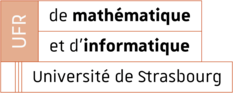
\includegraphics[height=0.85cm]{images/logo_ufr.png}}{}%
  \hspace{0.7cm}%
  \IfFileExists{images/cemosis-logo.png}%
    {
\includegraphics[height=0.85cm]{images/cemosis-logo.png}}{}%
  \par\vspace{1.2cm}%
}

\begin{document}

\maketitle


\begin{frame}{Outline}
  \tableofcontents
\end{frame}

\section{The problem and the protocol}

\begin{frame}{The problem}

  \centering

  \safeimage[width=0.88\linewidth]
  {../results/figures/record208_annotated.png}
  {Ten seconds of annotated ECG signal.}

  \vspace{0.5em}

  \begin{itemize}
    \item ECG recordings are mostly \textbf{normal}.
    \item Abnormal beats are \textbf{rare but important}.
    \item Goal: automatically flag beats that need a \textbf{second look}.
  \end{itemize}

  \vfill

  \sources{Moody \& Mark (2001); Goldberger et al. (2000).}

\end{frame}

\begin{frame}{Why anomaly detection, and where else it applies}

  \begin{columns}[T]

    \begin{column}{0.48\textwidth}
      \begin{block}{Why not plain classification}
        \begin{itemize}
          \item Abnormal events are rare and heterogeneous.
          \item Labels for every class may not exist in real monitoring.
          \item Anomaly detection models \emph{normal} behaviour and flags departures.
          \item MIT-BIH is fully annotated, so both settings run on the same beats.
        \end{itemize}
      \end{block}
    \end{column}

    \begin{column}{0.48\textwidth}
      ECG is the case study: vibration monitoring is the motivating analogy.

      \begin{block}{The same structure in industry}
        \begin{itemize}
          \item long time-series;
          \item mostly normal behaviour;
          \item rare abnormal events;
          \item few labels.
        \end{itemize}
      \end{block}
    \end{column}

  \end{columns}

  \keypoint{
  \begin{itemize}
    \item \textbf{Labels over model size}: Good supervision matters more than making the model larger.
    \item \textbf{Misleading averages}: Overall scores hide a clear drop in performance on the hardest class.
  \end{itemize}
  }

  \sources{Chandola et al. (2009); Ruff et al. (2021); Randall \& Antoni (2011); Lei et al. (2018).}

\end{frame}


\begin{frame}{Objectives}

  \begin{enumerate}
    \item Build a complete pipeline: raw ECG $\rightarrow$ one decision per heartbeat.
    \item Compare four levels of method on identical terms:
      statistical baselines, unsupervised models, supervised classifiers, autoencoders.
    \item Quantify what supervision contributes.
    \item Identify which arrhythmia classes remain difficult, and why.
    \item Deliver reproducible software: package, tests, CI, container.
  \end{enumerate}

  \keypoint{
    \vspace{0.1cm}
    The goal is a \textbf{rigorous, reproducible comparison}, not chasing an inflated metric.}

\end{frame}


\begin{frame}{Data: MIT-BIH and class imbalance}

  \begin{columns}[T]

    \begin{column}{0.52\textwidth}
      \centering
      \safeimage[height=0.62\textheight]
      {../results/figures/class_distribution.png}
      {Class distribution figure.}
    \end{column}

    \begin{column}{0.44\textwidth}

      \begin{tabular}{lrr}
        \toprule
        Class & Beats & Share \\
        \midrule
        N & 90\,631 & 82.8\% \\
        Q & 8\,043 & 7.3\% \\
        V & 7\,236 & 6.6\% \\
        S & 2\,781 & 2.5\% \\
        F & 803 & 0.7\% \\
        \bottomrule
      \end{tabular}

      \vspace{0.8em}

      \begin{itemize}
        \item 48 ECG recordings.
        \item About 109\,000 annotated heartbeats.
        \item Five AAMI groups: N, S, V, F, Q.
        \item About \textbf{113 normal beats per fusion beat}: accuracy is useless here.
      \end{itemize}

    \end{column}

  \end{columns}

  \sources{Moody \& Mark (2001); ANSI/AAMI EC57:2012.}

\end{frame}


\begin{frame}{Data: What must the model distinguish?}

  \centering

  \safeimage[width=0.86\textwidth]
  {../results/figures/beat_morphology.png}
  {Beat morphology figure.}

  \vfill

  \begin{itemize}
    \item Ventricular beats are wider and morphologically different: easy.
    \item Fusion beats blend normal and abnormal morphology.
    \item Supraventricular beats look almost normal: \textbf{timing is the only clue}.
  \end{itemize}

  \sources{de Chazal, O'Dwyer \& Reilly (2004); Luz et al. (2016).}

\end{frame}


\begin{frame}{Data: Preprocessing}

  \begin{columns}[T]

    \begin{column}{0.58\textwidth}
      \safeimage[width=\linewidth]
      {../results/statistical_baseline/figures/raw_vs_filtered.png}
      {Raw versus filtered ECG.}

      \keypoint{
        \vspace{0.1cm}
        R-peak positions come from annotations; beat detection itself is not evaluated.}

    \end{column}

    \begin{column}{0.38\textwidth}
      \begin{itemize}
        \item FFirst ECG lead: MLII (Modified Lead II).
        \item Band-pass filter: $0.5$--$10$ Hz, applied forwards and backwards.
        \item Beat centred on the annotated R-peak.
        \item Window:
        \[
          -0.25\,s \rightarrow +0.40\,s
        \]
        \item 234 samples per beat.
        \item Each record normalised independently.
      \end{itemize}
    \end{column}

  \end{columns}


\end{frame}


\begin{frame}{Evaluation protocol: fixed before any model was written}

  \begin{enumerate}
    \item \textbf{Decision unit:} one heartbeat.
    \item \textbf{Binary formulation:}
    \[
      N = \text{normal},
      \qquad
      S,V,F,Q = \text{anomaly}.
    \]
    \item \textbf{Inter-patient split:} DS1 = 22 training records, DS2 = 22 test records,
      no patient in both.
    \item Threshold selected on \textbf{DS1 only}, then frozen.
    \item Metrics: precision, recall, F1, ROC AUC. One module computes all of them.
  \end{enumerate}

  \sources{de Chazal, O'Dwyer \& Reilly (2004); Saito \& Rehmsmeier (2015).}

\end{frame}


\begin{frame}{Validation of the protocol}

  \begin{columns}[T]

    \begin{column}{0.45\textwidth}
      \centering
      \Large \textbf{Published DS2}\\[0.5em]
      \Huge 0.1097\\
      \normalsize anomaly rate
    \end{column}

    \begin{column}{0.10\textwidth}
      \centering
      \Huge $=$
    \end{column}

    \begin{column}{0.45\textwidth}
      \centering
      \Large \textbf{Our pipeline}\\[0.5em]
      \Huge \alert{0.1097}\\
      \normalsize anomaly rate
    \end{column}

  \end{columns}

  \vfill

 \begin{itemize}
  \item \textbf{Exact Match}: Our pipeline matches the published benchmark test set at exactly $10.97\%$ anomalies.
  \item \textbf{Clean Data Setup}: Confirms our patient split, filtering, and labels are 100\% correct before testing.
\end{itemize}

  \sources{de Chazal, O'Dwyer \& Reilly (2004).}

\end{frame}

\section{Methods, from a threshold to a neural network}

\begin{frame}{Statistical baselines: useful failures}

      \centering
      \small
      \begin{tabular}{lrrrr}
        \toprule
        Method & Prec. & Rec. & F1 & AUC \\
        \midrule
        Spectral & 0.297 & 0.502 & \good{0.373} & 0.773 \\
        CUSUM & 0.410 & 0.335 & 0.369 & 0.680 \\
        Z-score 10 s & 0.652 & 0.175 & 0.276 & 0.615 \\
        % ---- FIX: the random row is what makes the last row readable ----
        \textit{Random baseline} & 0.110 & 0.996 & \textit{0.198} & \textit{0.500} \\
        Z-score 1 s & 0.110 & 0.997 & 0.198 & \alert{0.274} \\
        \bottomrule
      \end{tabular}

      \normalsize
      \vspace{0.8em}

      \begin{itemize}
        \item The one-second window scores \textbf{below chance}: the beat becomes part of
          its own reference.
        \item The time window matters: a poor choice can reverse the result.
      \end{itemize}


  \sources{Page (1954) for CUSUM.}

\end{frame}


\begin{frame}{Engineered features and label-free models}

  \begin{columns}[T]

    \begin{column}{0.5\textwidth}
      \safeimage[width=\linewidth]
      {../results/features_unsupervised/figures/scalogram_normal_vs_v.png}
      {Scalogram: normal versus ventricular beat.}
    \end{column}

    \begin{column}{0.50\textwidth}

      \begin{itemize}
        \item 35 features per beat:
          9 rhythm, 10 morphological, 6 spectral, 10 wavelet.
        \item Two label-free models: Isolation Forest and One-Class SVM.
      \end{itemize}

      \vspace{0.4em}

      \begin{tabular}{lrrr}
        \toprule
        Method & Prec. & Rec. & F1 \\
        \midrule
        Isolation Forest & 0.343 & 0.566 & \good{0.427} \\
        One-Class SVM & 0.200 & 0.437 & 0.275 \\
        \bottomrule
      \end{tabular}

      \vspace{0.6em}
      {\small 35 features beat one hand-picked number by $+0.054$ F1.}

    \end{column}

  \end{columns}

  \sources{Liu, Ting \& Zhou (2008); Schölkopf et al. (2001); Mallat (1989); Addison (2005).}

\end{frame}


\begin{frame}{Supervised classification}

  \begin{columns}[T]

    \begin{column}{0.55\textwidth}
      \centering
      % NOTE: re-export this figure with a wider left margin,
      % the feature names are currently truncated (see notes)
      \safeimage[height=0.63\textheight]
      {../results/supervised_ml/figures/shap_importance.png}
      {SHAP feature importance.}
    \end{column}

    \begin{column}{0.45\textwidth}

      \begin{itemize}
        \item The same 35 features. The only change is access to labels.
        \item Random Forest and XGBoost, tuned with \textbf{grouped} cross-validation.
        \item SHAP: the four leading features are all \textbf{rhythm} features.
          Nobody told the model that; it agrees with a cardiologist.
      \end{itemize}

      \vspace{0.4em}

      \begin{tabular}{lrrr}
        \toprule
        Method & Prec. & Rec. & F1 \\
        \midrule
        Random Forest & 0.837 & 0.633 & \good{0.721} \\
        XGBoost & 0.686 & 0.677 & 0.681 \\
        \bottomrule
      \end{tabular}

    \end{column}

  \end{columns}

  \sources{Breiman (2001); Chen \& Guestrin (2016); Lundberg \& Lee (2017).}

\end{frame}


\begin{frame}{Autoencoders: reconstruction error as anomaly score}

  \begin{columns}[T]

    \begin{column}{0.50\textwidth}
      \safeimage[width=\linewidth]
      {../results/autoencoders/figures/cnn_reconstructions.png}
      {CNN reconstruction examples.}
    \end{column}

    \begin{column}{0.46\textwidth}

      \begin{itemize}
        \item Trained only on normal beats.
        \item The model learns to reconstruct normal ECG beats.
        \item A large reconstruction error suggests an anomaly.
        \item Two models: CNN and LSTM.
      \end{itemize}

      \vspace{0.4em}

      \begin{tabular}{lrrr}
        \toprule
        Method & Prec. & Rec. & F1 \\
        \midrule
        CNN  & 0.349 & 0.669 & \good{0.459} \\
        LSTM & 0.308 & 0.426 & 0.357 \\
        \bottomrule
      \end{tabular}

    \end{column}

  \end{columns}

  \sources{Sakurada \& Yairi (2014); Hochreiter \& Schmidhuber (1997).}

\end{frame}


\begin{frame}{Why training on normal beats matters}

  \begin{columns}[T,onlytextwidth]

    % Left: figure
    \begin{column}{0.52\textwidth}
      \safeimage[width=\linewidth]
      {../results/autoencoders/figures/cnn_error_distribution.png}
      {CNN reconstruction-error distributions.}

      \vspace{0.3em}
      \centering
      \small
      Normal and abnormal beats should have different reconstruction errors.

      \keypoint{
        \vspace{0.1em}
        For anomaly detection, the autoencoder should learn from normal beats only.}

    \end{column}

    % Right: results and explanation
    \begin{column}{0.44\textwidth}

      \centering
      \begin{tabular}{lcc}
        \toprule
        Training data & F1 & AUC \\
        \midrule
        Normal beats only & \good{0.459} & 0.839 \\
        All beats & \alert{0.171} & 0.708 \\
        Random baseline & 0.198 & 0.500 \\
        \bottomrule
      \end{tabular}

      \vspace{0.9em}

      \begin{itemize}
        \item The model and the amount of data stay the same.
        \item Only the \textbf{training data} changes.
        \item If the model sees abnormal beats during training, it learns to reconstruct them too.
        \item Then reconstruction error is less useful for detecting anomalies.
      \end{itemize}

      


    \end{column}

  \end{columns}

\end{frame}


\begin{frame}{Software: why the comparison can be trusted}

  \begin{columns}[T]

    \begin{column}{0.54\textwidth}
      \centering
      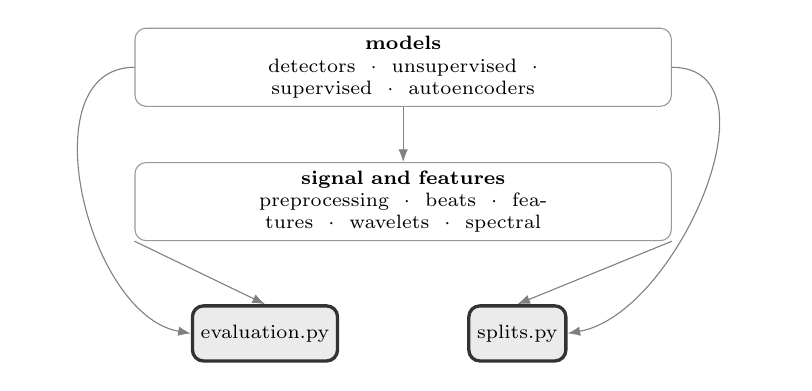
\begin{tikzpicture}[
          font=\scriptsize,
          box/.style={draw=black!40, rounded corners, align=center,
                      minimum height=0.7cm, inner sep=3pt},
          core/.style={box, very thick, draw=black!80, fill=black!8},
          arr/.style={-{Latex[length=1.6mm]}, gray}
        ]
        \node[box, text width=6.6cm] (models)
          {\textbf{models} \\ detectors \ $\cdot$ \ unsupervised \ $\cdot$ \ supervised \ $\cdot$ \ autoencoders};
        \node[box, text width=6.6cm, below=0.7cm of models] (feat)
          {\textbf{signal and features} \\ preprocessing \ $\cdot$ \ beats \ $\cdot$ \ features \ $\cdot$ \ wavelets \ $\cdot$ \ spectral};
        \node[core, below left=0.8cm and -2.6cm of feat] (eval) {evaluation.py};
        \node[core, below right=0.8cm and -2.6cm of feat] (split) {splits.py};

        \draw[arr] (models) -- (feat);
        \draw[arr] (feat.south west) -- (eval.north);
        \draw[arr] (feat.south east) -- (split.north);
        \draw[arr] (models.west) to[out=180, in=170] (eval.west);
        \draw[arr] (models.east) to[out=0, in=10] (split.east);
      \end{tikzpicture}

      \vspace{0.4em}
      {\scriptsize Every arrow points downwards: the two core modules import nothing.}
    \end{column}

    \begin{column}{0.42\textwidth}
      \begin{itemize}
        \item \textbf{One} function computes F1. \textbf{One} function chooses a threshold.
          No method can be measured on different terms from another.
        \item Automated tests check that the code works correctly.
        \item CI on every push; the DS1/DS2 leakage checks run on every commit.
        \item Installable package and published container image.
      \end{itemize}
    \end{column}

  \end{columns}

  \keypoint{
    \vspace{0.1em}
    The software is a result, not scaffolding: it is what makes the ranking believable.}

\end{frame}

\section{What supervision buys, and what the average hides}

\begin{frame}{Overall comparison: performance and cost}

  \centering
  \small

  \begin{tabular}{lccccc}
    \toprule
    Method & Labels & Prec. & Rec. & F1 & Cost (min) \\
    \midrule
    Random Forest & yes & \good{0.837} & 0.633 & \good{0.721} & $<0.1$ \\
    XGBoost & yes & 0.686 & \good{0.677} & 0.681 & $<0.1$ \\
    CNN autoencoder & no & 0.349 & 0.669 & 0.459 & 6.5 \\
    Isolation Forest & no & 0.343 & 0.566 & 0.427 & $<0.1$ \\
    Spectral features & no & 0.297 & 0.502 & 0.373 & $<0.1$ \\
    LSTM autoencoder & no & 0.308 & 0.426 & 0.357 & 17.2 \\
    \bottomrule
  \end{tabular}

  \vspace{0.3em}
  {\scriptsize All timings on a laptop CPU, no GPU.}

  \vfill

  \begin{columns}[T]

    \begin{column}{0.48\textwidth}
      \begin{itemize}
        \item Supervised models are clearly ahead.
        \item Cost and accuracy do not move together.
      \end{itemize}
    \end{column}

    \begin{column}{0.48\textwidth}
      \begin{itemize}
        \item The CNN gains $0.032$ F1 over Isolation Forest\ldots
        \item \ldots for roughly 100 times the computation.
      \end{itemize}
    \end{column}

  \end{columns}


\end{frame}


\begin{frame}{What do labels improve?}

  \centering

  % Main comparison table
  \begin{tabular}{lccc}
    \toprule
    Method & Precision & Recall & F1 \\
    \midrule
    Isolation Forest & 0.343 & 0.566 & 0.427 \\
    Random Forest    & \good{0.837} & 0.633 & \good{0.721} \\
    \midrule
    Improvement      & \alert{+0.494} & +0.067 & +0.294 \\
    \bottomrule
  \end{tabular}

  \vspace{1.2em}

  \begin{columns}[T,onlytextwidth]

    \begin{column}{0.47\textwidth}
      \begin{itemize}
        \item Both models use the same 35 features.
        \item The biggest improvement is in \textbf{precision}.
      \end{itemize}
    \end{column}

    \begin{column}{0.47\textwidth}
      \begin{itemize}
        \item Labels help reduce false alarms.
        \item Recall improves only a little.
      \end{itemize}
    \end{column}

  \end{columns}

  \vfill

  \keypoint{\vspace{0.1cm}
  Labels mainly help the model avoid false alarms.}

\end{frame}


\begin{frame}{How certain are these differences?}

  \begin{columns}[T]

    \begin{column}{0.43\textwidth}
      \centering

      \Huge 49\,692\\
      \normalsize beats in DS2

      \vspace{1em}

      \Huge $\neq$

      \vspace{1em}

      \Huge \alert{22}\\
      \normalsize independent patients
    \end{column}

  \begin{column}{0.56\textwidth}

    \begin{itemize}
      \item Beats from the same patient are related.
      \item So the number of \textbf{patients} matters more than the number of beats.
    \end{itemize}

    \vspace{0.5em}

    \textbf{Small difference:}

    \[
      0.459 - 0.427 = 0.032
    \]

    \centering
    Too small to make a strong claim.

    \vspace{0.8em}

    \raggedright
    \textbf{Larger differences:}
    \begin{itemize}
      \item Supervision: \textbf{+0.294 F1}
      \item Autoencoder ablation: \textbf{0.459 $\rightarrow$ 0.171}
    \end{itemize}

  \end{column}

  \end{columns}

  \keypoint{
    \vspace{0.1cm}
    Focus on the big differences, not every decimal.}

\end{frame}


\begin{frame}{Per-class recall: different models catch different beats}

\centering

\small
\begin{tabular}{lcccc}
  \toprule
  Method & Labels & S & V & F \\
  \midrule
  Random Forest    & yes & 0.161 & \good{0.946} & 0.281 \\
  XGBoost          & yes & 0.275 & \good{0.946} & \good{0.351} \\
  CNN autoencoder  & no  & \alert{0.654} & 0.750 & 0.064 \\
  LSTM autoencoder & no  & 0.484 & 0.441 & 0.018 \\
  Isolation Forest & no  & 0.380 & 0.717 & 0.106 \\
  \bottomrule
\end{tabular}

\vspace{1em}

\begin{columns}[T,onlytextwidth]

  \begin{column}{0.47\textwidth}
    \begin{block}{Supervised models}
      \begin{itemize}
        \item Very strong on \textbf{ventricular beats (V)}.
        \item Random Forest and XGBoost detect about \textbf{95\%} of them.
      \end{itemize}
    \end{block}
  \end{column}

  \begin{column}{0.47\textwidth}
    \begin{block}{Label-free models}
      \begin{itemize}
        \item Better on \textbf{supraventricular beats (S)}.
        \item CNN autoencoder reaches \textbf{0.654 recall}.
      \end{itemize}
    \end{block}
  \end{column}

\end{columns}

\vspace{0.6em}

\centering
\textbf{Fusion beats (F) remain difficult for all methods.}

\vfill

\keypoint{The best overall model is not the best for every class.}

\end{frame}

\section{Limits and outlook}


\begin{frame}{Limitations}

  \begin{columns}[T]
    \begin{column}{0.48\textwidth}
      \begin{block}{What the numbers assume}
        \begin{itemize}
          \item \textbf{R-peaks are given} by expert annotations; no detection stage is
            evaluated, so every score is optimistic.
          \item One database, one lead, no pacemaker patients.
          \item Each beat is evaluated separately, without using the surrounding beats.
        \end{itemize}
      \end{block}
    \end{column}
    \begin{column}{0.48\textwidth}
      \begin{block}{What the system does not claim}
        \begin{itemize}
          \item It flags suspicious beats; it does not diagnose.
          \item Fusion beats defeat every method here.
          \item The LSTM memorises its training patients (validation error four times
            the training error).
        \end{itemize}
      \end{block}
    \end{column}
  \end{columns}

  \keypoint{
    \vspace{0.1cm}
    The results hold for beat windows whose R-peak positions are already known
  to be correct.}

\end{frame}


\begin{frame}{Conclusion and perspectives}

  \begin{columns}[T]

    \begin{column}{0.48\textwidth}
      \begin{block}{What was established}
        \begin{enumerate}
          \item A complete, reproducible pipeline, protocol fixed before any model.
          \item Supervised models give the best global F1, and the gain is precision.
          \item Label-free models catch the rare beats the others ignore.
          \item With 22 test patients, small gaps mean nothing and are not claimed.
        \end{enumerate}
      \end{block}
    \end{column}

    \begin{column}{0.48\textwidth}
      \begin{block}{Where it goes next}
        \begin{enumerate}
          \item \textbf{Combine the two families} --- the clearest lead, already worth
            recall 0.726 between two autoencoders alone.
          \item Add a real R-peak detector and close the pipeline.
          \item Repeat the protocol on a second database.
          \item Thresholds per patient, or from clinical cost rather than F1.
          \item Carry the method to vibration signals.
        \end{enumerate}
      \end{block}
    \end{column}

  \end{columns}

  \keypoint{
  For rare-event detection the average score is not enough: the protocol, the
  uncertainty and the per-class errors decide what it means.}

\end{frame}


\begin{frame}[standout]
  Thank you for your attention.

  \vspace{1em}

  Questions?
\end{frame}



\end{document}